% ----------------------------------------
% Chap: 
% ----------------------------------------
\chapter{Durchgeführte experimentellen Methoden zur Schmierfilmdickenmessung}
\label{chap:durchgefuehrte_experimentellen_methoden}

% ----------------------------------------
% Sec: 
% ----------------------------------------
\section{PCS Instrument Prüfstand}
\label{sec:pcs_pruefstand}

Zur Schmierfilmdickenmessung wurde ein ``EHL Ultra Thin Film Measurement System'' der Firma PCS-Instrument genutzt (Abbildung \ref{fig:ehl_messgeraet}).
Basiert auf dem Kugel-Scheibe-Modell und optischer Interferenz wird die Schmierfilmdicke im EHD-Kontakt ermittelt.
Durch einen leicht modifizierten Aufbau, ermöglicht das Gerät auch die Bestimmung von Reibkoeffizienten der eingesetzten Schmierstoffe.
Im Folgenden wird kurz auf die einzelnen Komponenten des EHL-Gerätes und die Modifikation im Rahmen dieser Arbeit eingegangen.

% ----------------------------------------
% Fig: EHL Prüfstand
% ----------------------------------------
\begin{figure}[htb]
    \centering
    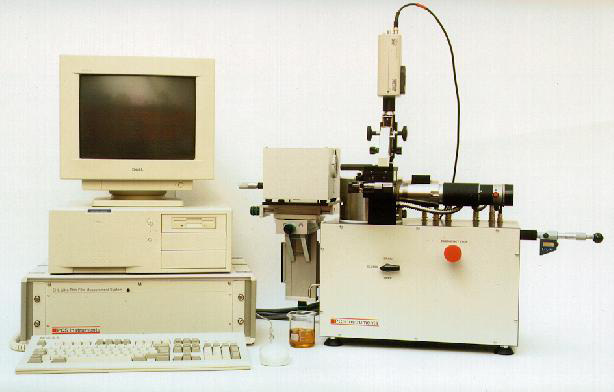
\includegraphics[width=0.8\linewidth]{./images/ehl_pruefstand.png}
    \caption{EHL-Messgerät \cite{ehl}}
    \label{fig:ehl_messgeraet}
\end{figure}

% ----------------------------------------
% Sec: 
% ----------------------------------------
\subsection{PC und Elektronikeinheit}
\label{sub:pc_elektronikeinheit}

Zur Bedienung des Prüfstands steht einen PC zur Verfügung.
Der PC hat Windows 98 als Betriebssystem und fünf ISA-Steckkarten.
Diese Karten sind für die Ein-/Ausgabe, die Zeiterfassung, die SW-Bilderfassung sowie ADC und DAC zuständig.
Die Kommunikation mit dem Prüfstand erfolgt durch das Softwarepaket ``Ultra Thin Film EHL Measurement''.
Der PC ist mit einem Spektrometer, einem SW-Monitor und einer Elektronikeinheit verbunden.

Zu der Elektronikeinheit gehören die Motoren, die Lasteinheit sowie die Heizvorrichtung.
Außerdem ist eine Überwachungsfunktion eingebaut, die beim einem Absturz der Software oder des PC den Prüfstand abschaltet.

% ----------------------------------------
% Sec: Meschanischer Aufbau
% ----------------------------------------
\subsection{Mechanischer Aufbau}
\label{sub:mechanischer_aufbau}

Abbildung \ref{fig:ehl_aufbau} zeigt den Schematischen Aufbau des EHL-Prüfstands.
Das Reservoir ist bei Messungen mit Öl bis die Hälfte der Kugel gefüllt.
Durch die Heizvorrichtung kann das Öl bis c.a $150 ^\circ C$ temperiert werden.
% ----------------------------------------
% Fig: EHL Aufbau
% ----------------------------------------
\begin{figure}[htb]
    \centering
    
\includegraphics[width=4cm]{./images/blank_img.jpg}
    \caption{Schematischer Aufbau des EHL-Prüfstands \cite{ehl}}
    \label{fig:ehl_aufbau}
\end{figure}
%
Der elastohydrodynamische Schmierfilm wird durch einen Kugel-Scheibe-Kontakt erzeugt.
Die Kugel ist hochglanzpoliert, aus 100Cr6 Stahl und hat einen Durchmesser von 19,05 mm.
Es gibt zwei Variationen der Kugel, normal und durchgebohrt.
Über ein Kugel-Support wird die Kugel von unten von eine Lasteinheit gegen einer sich rotierenden Glasscheibe gedrückt.
Die Last ist von 0-50 N wählbar und ergibt sich einen maximalen Druck von 0,7 GPa im Kontaktpunkt.
Die Glasscheibe hat einen Durchmesser von 100 mm und ist an der Unterseite mit einer durchlässigen Chromschicht und einer Silikatschicht zu versehen.
Es gibt insgesamt 21 befahrbaren Spuren (R = $34 \rightarrow 44$ mm) auf der Scheibe durch die axiale Verschiebung des Kugel-Supports.
Ein Spurwechsel ist nötig, weil die Silikatschicht, die nicht so robust sowie die Chromschicht ist, mit Laufe der Zeit abgenutzt wird.

Die Scheibe kann von 1 mm/s bis 5 m/s durch einen Motor betrieben werden.
Ein weiterer Motor ermöglicht auch das Antreiben der Kugel.
In diesem Fall sind Versuche mit Schlüpf zwischen Kugel und Scheibe innerhalb von 0 - 200 \% ermöglicht.

Das originale Kugel-Support von PCS-Instrument besteht aus drei Lager, die auf einem dreieckigen Aluminium-Klotz geschraubt werden.
Eine modifizierte Lagerung mit einstellbarer, geführte Achse von Wittek \cite{wittek_2007} steht auch zur Verfügung (Abbildung \ref{fig:kugel_support}).
% ----------------------------------------
% Fig: Kugel-Support
% ----------------------------------------
\begin{figure}[htb]
    \centering

    \begin{subfigure}[b]{0.3\textwidth}
        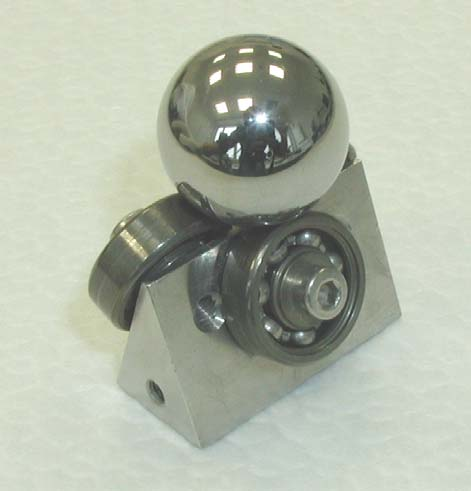
\includegraphics[width=\textwidth]{./images/kugel-support_original.png}
    \end{subfigure}
    %
    \begin{subfigure}[b]{0.3\textwidth}
        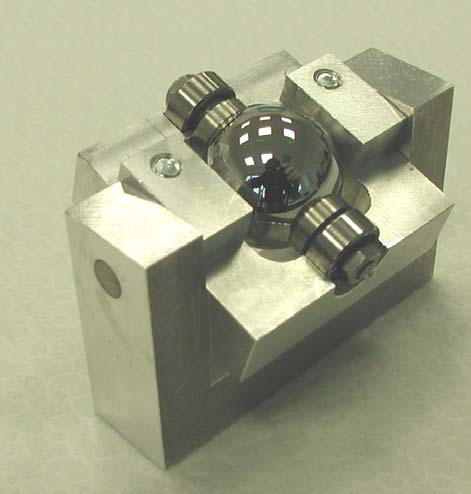
\includegraphics[width=\textwidth]{./images/kugel-support_wittek.png}
    \end{subfigure}
    \caption{Originaler PCS-Support (links) und modifizierter Support (rechts) \cite{wittek_2007}}
    \label{fig:kugel_support}
\end{figure}
%

\improvement[inline]{Prüfstand Spezifikation}

% ----------------------------------------
% Sec: 
% ----------------------------------------
\subsection{Messsystem zur Schmierfilmdickemessung}
\label{sub:messsystem_zur_schmierfilmdickemessung}

% ----------------------------------------
% Sec: 
% ----------------------------------------
\section{Versuchte Öle}
\label{sec:versuchte_oele}

% ----------------------------------------
% Sec: 
% ----------------------------------------
\section{Versuchdurchführung}
\label{sec:versuchdurchfuehrung}
